\documentclass[a4paper,12pt,openany]{book}


\usepackage[utf8]{inputenc}
\usepackage[T1]{fontenc}
\usepackage[bahasa]{babel}
\usepackage{geometry}
\geometry{
 a4paper,
 left=20mm,
 right=20mm,
 top=20mm,
 bottom=20mm,
}

\usepackage{microtype}
\usepackage{graphicx}
\usepackage{booktabs}
\usepackage{hyperref}
\usepackage{titlesec}
\usepackage{titling}
\usepackage{amsmath}
\usepackage{fancyhdr}
\usepackage{setspace}
\usepackage{biblatex}
\usepackage{titlesec}
\usepackage{listings}
\usepackage{float}
\usepackage{indentfirst}

\titlespacing*{\chapter}{0pt}{-50pt}{40pt}

\addbibresource{references.bib}

\pretitle{\begin{flushleft}\Huge\bfseries}
\posttitle{\par\end{flushleft}\vskip 10em}

\preauthor{\begin{flushleft}\large}
\postauthor{\end{flushleft}}

\pagestyle{fancy}
\fancyhf{}
\fancyhead[L]{\leftmark}
\renewcommand{\headrulewidth}{0pt}

\title{Operasi-Operasi Dasar \\Pengolahan Citra}
\author{
\begin{tabbing}
Disusun Oleh : \\ Helmy Luqmanulhakim \hspace{5em} \= 22051204014 \\
\end{tabbing}
\vspace{5em}
\begin{flushleft}
\textbf{Pengolahan Citra Digital} \vspace{0.2em} \\
\textbf{S1 Teknik Informatika} \vspace{0.2em} \\
\textbf{Fakultas Teknik} \vspace{0.2em} \\
\textbf{Universitas Negeri Surabaya} \vspace{0.2em}\\
\textbf{2024} \vspace{0.2em}
\end{flushleft}
}
\date{}

\begin{document}

\maketitle
\thispagestyle{fancy}

\tableofcontents

...


\chapter{Pendahuluan}


Pengolahan citra adalah proses penting dalam dunia digital di mana citra-citra diproses untuk berbagai tujuan, seperti meningkatkan kualitasnya, mengekstrak informasi yang berguna, atau mengubahnya agar lebih mudah dipahami baik oleh manusia maupun mesin. Dalam pengolahan citra, terdapat beberapa tingkatan operasi yang umum digunakan, yang dapat dibagi menjadi empat level komputasi:

\begin{enumerate}
    \item \textbf{Level Piksel} \
          Ini adalah level paling dasar dalam pengolahan citra, di mana operasi dilakukan pada setiap piksel citra. Pada level ini, sering dilakukan operasi aritmatika, logika, dan geometri.
    \item \textbf{Level Lokal} \
          Pada level ini, operasi dilakukan pada sekelompok piksel, yang merupakan level yang lebih tinggi dari level piksel. Operasi yang sering dilakukan di sini adalah operasi konvolusi.
    \item \textbf{Level Global} \
          Ini adalah level yang lebih tinggi dari level lokal, di mana operasi dilakukan pada seluruh piksel citra. Operasi yang sering dilakukan di level ini adalah operasi histogram.
    \item \textbf{Level Objek} \
          Ini adalah level paling tinggi, di mana operasi dilakukan pada objek yang ada dalam citra. Operasi yang sering dilakukan di sini adalah segmentasi.
\end{enumerate}

\subsection{Operasi Aritmatika}

Pada dasarnya, operasi aritmatika merujuk pada serangkaian manipulasi matematis yang diterapkan pada setiap piksel dalam suatu citra. Ini mirip dengan menyelami setiap titik dalam gambar dan melakukan perhitungan tertentu untuk mengubahnya. Kita bisa membayangkan ini sebagai proses yang mirip dengan memberikan sentuhan artistik pada lukisan digital kita. Misalnya, dengan menggunakan operator matematika seperti penambahan, pengurangan, perkalian, atau pembagian, kita dapat mengatur kontras dalam citra untuk membuatnya lebih tajam atau memperbaiki kecerahan agar terlihat lebih seimbang.



\subsection{Operasi Logika}

Operasi logika merupakan serangkaian manipulasi yang diterapkan pada setiap piksel dalam citra menggunakan operator logika seperti AND, OR, dan NOT. Konsepnya mirip dengan mengadakan perbandingan piksel demi piksel untuk menentukan pola atau keadaan tertentu. Misalnya, dengan menggunakan operator AND, kita bisa menggabungkan dua citra untuk menciptakan citra baru yang mewakili kesamaan antara keduanya. Sementara itu, operator OR dapat digunakan untuk menciptakan citra baru yang memuat informasi dari salah satu citra atau keduanya. Sedangkan operator NOT memungkinkan kita untuk membalik piksel, mengubah area yang gelap menjadi terang dan sebaliknya.

Operasi logika ini tidak hanya berguna untuk penggabungan atau pemisahan citra, tetapi juga untuk mengubah bentuk atau memperjelas detail dalam citra. Misalnya, dengan memanfaatkan operator logika, kita dapat mengekstraksi garis-garis atau bentuk-bentuk tertentu dari citra, membuatnya lebih mudah diproses atau dianalisis lebih lanjut. Dengan demikian, operasi logika memberikan alat yang kuat untuk manipulasi citra yang memungkinkan pengguna untuk mengeksplorasi berbagai aspek visual dengan lebih mendalam dan kreatif.

\subsection{Operasi Geometri}

Operasi geometri merupakan proses yang melibatkan manipulasi setiap piksel dalam citra menggunakan operator geometri seperti translasi, rotasi, dan scaling. Ini adalah cara untuk memindahkan, memutar, atau mengubah skala citra untuk mencapai efek visual yang diinginkan. Misalnya, translasi memungkinkan kita untuk memindahkan seluruh citra ke arah yang ditentukan, menggeser posisi relatif setiap piksel. Rotasi memungkinkan kita untuk memutar citra sekitar titik tertentu, sementara scaling memungkinkan kita untuk memperbesar atau memperkecil citra secara proporsional.

Operasi geometri ini dapat digunakan untuk berbagai tujuan, seperti mengubah bentuk objek dalam citra, memperbaiki distorsi, atau bahkan menciptakan efek artistik yang unik. Misalnya, dengan memanfaatkan rotasi, kita dapat menyusun ulang orientasi objek dalam citra untuk menciptakan tampilan yang lebih dinamis. Begitu pula dengan scaling, kita dapat memperbesar bagian tertentu dari citra untuk menyoroti detail atau memperkecilnya untuk menciptakan efek jarak jauh. Dengan demikian, operasi geometri memberikan alat yang kuat untuk mengubah tampilan citra sesuai dengan kebutuhan dan preferensi pengguna.

\subsection{Operasi Histogram}

Operasi histogram adalah proses yang melibatkan analisis distribusi intensitas piksel dalam citra. Ini adalah cara untuk memahami bagaimana intensitas piksel didistribusikan dalam citra, yang dapat memberikan wawasan yang berharga tentang karakteristik visualnya. Misalnya, dengan menggunakan histogram, kita dapat melihat seberapa seragam intensitas piksel dalam citra, seberapa banyak piksel yang memiliki intensitas tertentu, atau seberapa jauh distribusi intensitasnya dari nilai rata-rata.

Operasi histogram ini berguna untuk berbagai tujuan, seperti penyesuaian kontras, peningkatan kecerahan, atau bahkan segmentasi citra. Misalnya, dengan memanfaatkan histogram, kita dapat menentukan apakah citra memiliki kontras yang cukup atau apakah ada area yang terlalu gelap atau terlalu terang. Dengan demikian, operasi histogram memberikan alat yang kuat untuk menganalisis dan memahami karakteristik visual citra, yang memungkinkan pengguna untuk membuat penyesuaian yang tepat sesuai dengan kebutuhan dan preferensi mereka.

\subsection{Operasi Segmentasi}

Operasi segmentasi adalah proses yang melibatkan pemisahan citra menjadi bagian-bagian yang lebih kecil atau lebih terdefinisi. Ini adalah cara untuk mengidentifikasi dan mengekstraksi objek atau area tertentu dalam citra, yang memungkinkan kita untuk memahami dan menganalisis informasi yang terkandung di dalamnya. Misalnya, dengan menggunakan segmentasi, kita dapat memisahkan objek dari latar belakang, mengidentifikasi area tertentu dalam citra, atau bahkan menentukan batas-batas antara objek yang berdekatan.

Operasi segmentasi ini berguna untuk berbagai tujuan, seperti pengenalan pola, analisis medis, atau bahkan pemrosesan gambar satelit. Misalnya, dengan memanfaatkan segmentasi, kita dapat mengidentifikasi area tertentu dalam citra yang memiliki karakteristik visual tertentu, seperti warna, tekstur, atau bentuk. Dengan demikian, operasi segmentasi memberikan alat yang kuat untuk mengidentifikasi dan mengekstraksi informasi yang berguna dari citra, yang memungkinkan pengguna untuk membuat analisis yang lebih mendalam dan akurat.

\section{Tujuan}

Dalam laporan ini, kita menyelami dunia yang menakjubkan dari pengolahan citra, menggali ke dalam keajaiban operasi-operasi dasar yang membentuk inti dari proses ini. Tujuan utama kita adalah untuk membawa Anda dalam perjalanan mendalam, mempersembahkan pemahaman yang lebih dalam tentang bagaimana citra dapat diubah dan diperbaiki melalui operasi-operasi seperti aritmatika, logika, dan geometri. Melalui lensa bahasa pemrograman Rust, kita akan menelusuri bagaimana setiap operasi ini dapat direplikasi dan diterapkan dalam kode, dengan bantuan pustaka image yang memungkinkan kita menjelajahi kemungkinan-kemungkinan baru.

\section{Metode}

Pendekatan penulis dalam laporan ini adalah menjelajahi konsep-konsep mendasar di balik manipulasi citra, membenamkan diri dalam pemahaman tentang alur dan implikasi dari setiap operasi yang digunakan. penulis tidak hanya memperkenalkan konsep tersebut secara sekilas, tetapi juga merenungkan tentang cara terbaik untuk menerapkannya menggunakan bahasa pemrograman Rust.

\section{Ruang Lingkup}

Jangkauan laporan ini melampaui sekedar pengenalan singkat tentang operasi-operasi dasar dalam pengolahan citra. penulis menelusuri ke dalam keunikan masing-masing operasi, membedahnya secara rinci dan menggambarkan dampaknya pada citra yang dihasilkan. Dari operasi aritmatika yang mengubah intensitas warna hingga operasi geometri yang memanipulasi struktur spasial, penulis mengeksplorasi berbagai aspek pengolahan citra dengan kedalaman yang memikat. Dan melalui perangkat bahasa pemrograman Rust dan pustaka image, penulis mengundang Anda untuk merasakan kekuatan kreatif yang terkandung di dalamnya, membuka jalan bagi eksplorasi tak terbatas dalam dunia pengolahan citra yang mempesona.

\chapter{Penerapan Operasi Dasar Pengolahan Citra}
\section{Penggunaan Operasi Aritmatika}
\subsection{Penambahan Citra}
Operasi penambahan citra adalah salah satu operasi aritmatika yang paling sederhana dan paling umum digunakan dalam pengolahan citra. Ide dasarnya adalah untuk menambahkan nilai piksel dari dua citra untuk menghasilkan citra baru yang mewakili kombinasi dari keduanya. Misalnya, dengan menambahkan dua citra yang mewakili cahaya merah dan cahaya biru, kita dapat menciptakan citra baru yang mewakili cahaya ungu. Dengan demikian, operasi penambahan citra memungkinkan kita untuk menggabungkan informasi dari dua citra untuk menciptakan citra baru yang lebih kaya dan bermakna.

\subsubsection{Contoh}
Misalnya, kita memiliki dua citra berikut:


\begin{figure}[H]
    \centering
    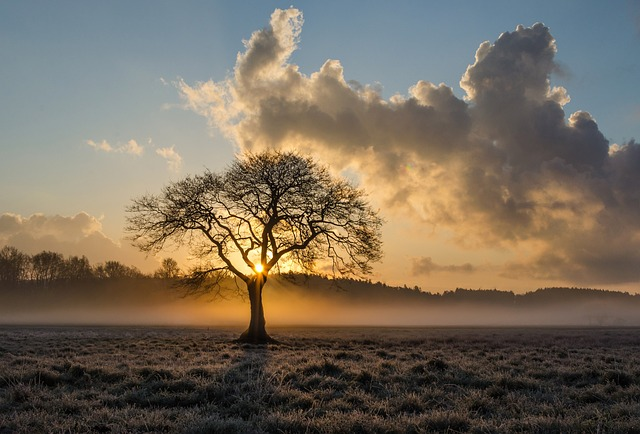
\includegraphics[width=0.4\textwidth]{./image/arithmetic/lone-tree.jpg}
    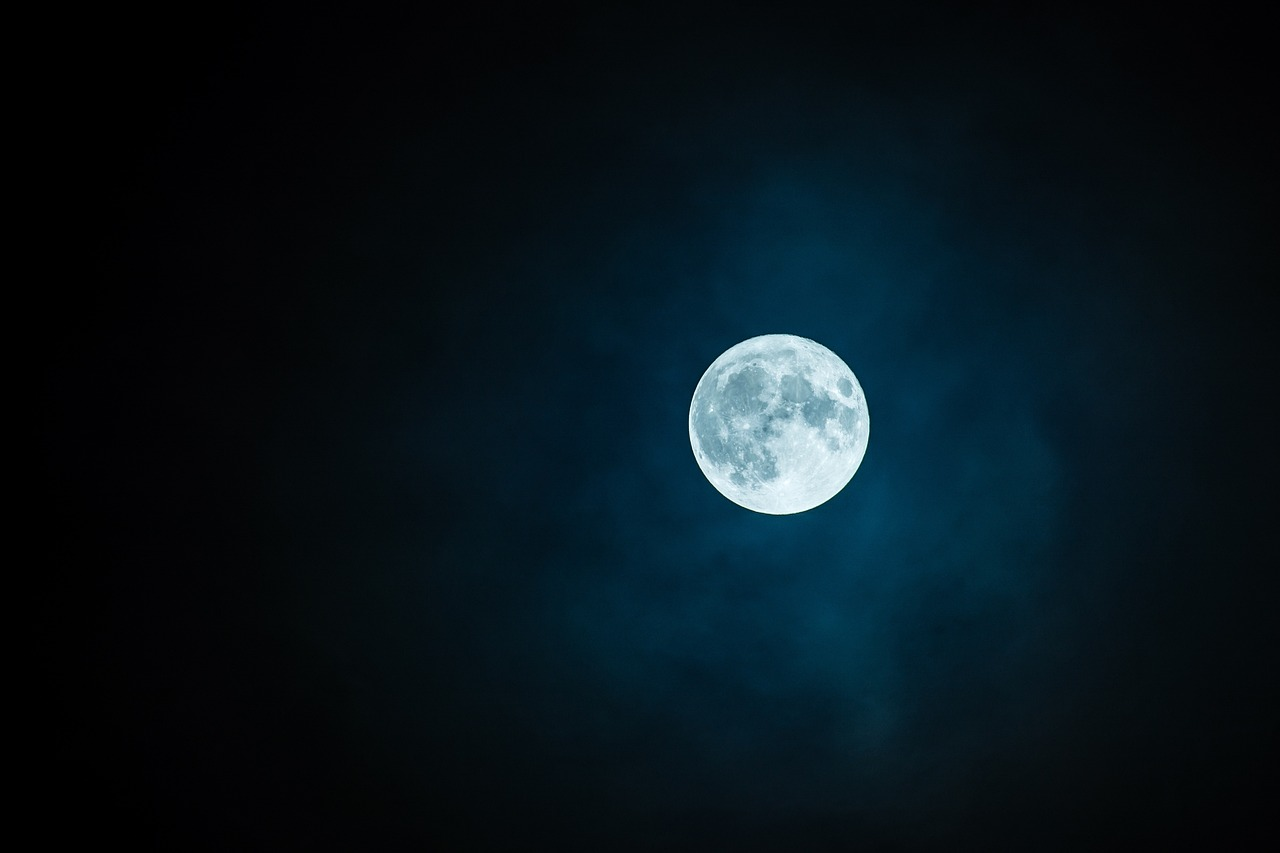
\includegraphics[width=0.4\textwidth]{./image/arithmetic/moon.jpg}
    \caption{Contoh Citra}
\end{figure}

Kita dapat menambahkan kedua citra ini menggunakan operasi penambahan citra untuk menciptakan citra baru yang mewakili kombinasi dari keduanya. Menggunakan Rust, kita dapat melakukan operasi ini dengan mudah menggunakan library image dengan kode berikut:

\begin{lstlisting}
use image::{open, GenericImageView, RgbaImage, Pixel, imageops};

fn main() {
    let tree = open("lone-tree.jpg").unwrap();
    let mut moon = open("moon.jpg").unwrap();

    let (width, height) = tree.dimensions();
    moon = image::DynamicImage::ImageRgba8(imageops::resize(&moon, width, height, imageops::FilterType::Nearest));

    let mut result = RgbaImage::new(width, height);

    for x in 0..width {
        for y in 0..height {
            let tree_pixel = tree.get_pixel(x, y);
            let moon_pixel = moon.get_pixel(x, y);
            let tree_channels = tree_pixel.channels();
            let moon_channels = moon_pixel.channels();
            let (r1, g1, b1, a1) = (tree_channels[0],
                                    tree_channels[1],
                                    tree_channels[2],
                                    tree_channels[3]);
            let (r2, g2, b2, a2) = (moon_channels[0],
                                    moon_channels[1],
                                    moon_channels[2],
                                    moon_channels[3]);
            let r = r1.saturating_add(r2);
            let g = g1.saturating_add(g2);
            let b = b1.saturating_add(b2);
            let a = a1.saturating_add(a2);
            result.put_pixel(x, y, image::Rgba([r, g, b, a]));
        }
    }

    result.save("result-addition.png").unwrap();
}
\end{lstlisting}

\begin{figure}[H]
    \centering
    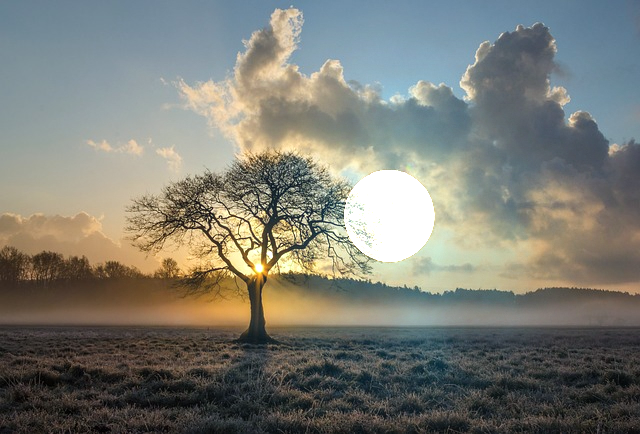
\includegraphics[width=0.4\textwidth]{./image/arithmetic/result-addition.png}
    \caption{Hasil Penambahan Citra}
\end{figure}

\subsection{Pengurangan Citra}
Operasi pengurangan citra adalah suatu teknik yang berguna dalam pemrosesan citra untuk mengekstraksi perbedaan antara dua gambar. Dengan cara ini, kita bisa mendapatkan pemahaman yang lebih dalam tentang informasi yang tersimpan dalam setiap gambar, serta mengungkapkan perbedaan yang mungkin tidak terlihat secara langsung. Misalnya, bayangkan kita memiliki dua foto, satu dengan cahaya merah yang mencolok dan yang lain dengan cahaya biru yang menarik. Dengan mengurangkan nilai piksel cahaya biru dari yang merah, kita dapat menghasilkan gambar baru yang menyoroti perbedaan warna tersebut. Ini bisa sangat berguna dalam berbagai aplikasi, dari analisis medis hingga pemrosesan gambar satelit.

\subsubsection{Contoh}
Misalnya, kita memiliki dua citra berikut:
\begin{figure}[H]
    \centering
    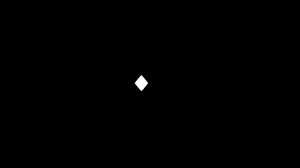
\includegraphics[width=0.4\textwidth]{./image/arithmetic/dot.jpg}
    
\includegraphics[width=0.4\textwidth]{./image/arithmetic/star-1.jpg}
    \caption{Contoh Citra}
\end{figure}

Sebagai contoh, mari kita ambil dua gambar, satu berisi titik dan yang lain berisi bintang. Dengan melakukan pengurangan citra, kita bisa menyoroti perbedaan antara kedua gambar tersebut, mungkin menunjukkan pola unik yang muncul dari perbedaan distribusi intensitas piksel. Implementasi operasi ini dengan Rust menggunakan library image memberikan akses yang mudah dan efisien untuk melakukan proses tersebut. Dengan cara ini, kita dapat menjelajahi dan menganalisis perbedaan visual antara gambar-gambar tersebut dengan lebih baik, membuka potensi baru untuk pemahaman dan interpretasi dalam berbagai konteks aplikasi.

\begin{lstlisting}
use image::{open, GenericImageView, RgbaImage, Pixel, imageops};

fn main() {
    let dot = open("dot.jpg").unwrap();
    let mut star = open("star-1.jpg").unwrap();

    let (width, height) = dot.dimensions();
    star = image::DynamicImage::ImageRgba8(imageops::resize(&star, width, height, imageops::FilterType::Nearest));

    let mut result = RgbaImage::new(width, height);

    for x in 0..width {
        for y in 0..height {
            let dot_pixel = dot.get_pixel(x, y);
            let star_pixel = star.get_pixel(x, y);
            let dot_channels = dot_pixel.channels();
            let star_channels = star_pixel.channels();
            let (r1, g1, b1, a1) = (dot_channels[0],
                                    dot_channels[1],
                                    dot_channels[2],
                                    dot_channels[3]);
            let (r2, g2, b2, a2) = (star_channels[0],
                                    star_channels[1],
                                    star_channels[2],
                                    star_channels[3]);
            let r = (r1 as i16 - r2 as i16).abs() as u8;
            let g = (g1 as i16 - g2 as i16).abs() as u8;
            let b = (b1 as i16 - b2 as i16).abs() as u8;
            let a = (a1 as i16 - a2 as i16).abs() as u8;
            result.put_pixel(x, y, image::Rgba([r, g, b, a]));
        }
    }

    result.save("result-subtraction.jpg").unwrap();
}
\end{lstlisting}

Kode di atas menggunakan operasi pengurangan citra untuk menciptakan citra baru yang mewakili perbedaan antara dua citra. Dalam contoh ini, kita menggunakan gambar bintang sebagai citra yang dikurangkan dari citra titik untuk mengekstraksi perbedaan antara keduanya.

\begin{figure}[H]
    \centering
    
\includegraphics[width=0.4\textwidth]{./image/arithmetic/result-subtraction.jpg}
    \caption{Hasil Pengurangan Citra}
\end{figure}

\subsection{Perkalian Citra}
Perkalian citra merupakan salah satu teknik penting dalam pemrosesan citra yang melibatkan operasi aritmatika sederhana, yaitu perkalian nilai piksel. Tujuan utamanya sering kali berkisar pada penerapan efek visual yang menarik dan pemrosesan citra yang lebih mendalam. Salah satu contoh penerapannya adalah dalam teknik yang disebut sebagai \textit{Image Masking}, di mana sebuah citra dikalikan dengan sebuah maska (matriks) yang memiliki ukuran lebih kecil daripada citra asli.

\subsubsection{Contoh}
Misalnya, kita memiliki citra berikut:
\begin{figure}[H]
    \centering
    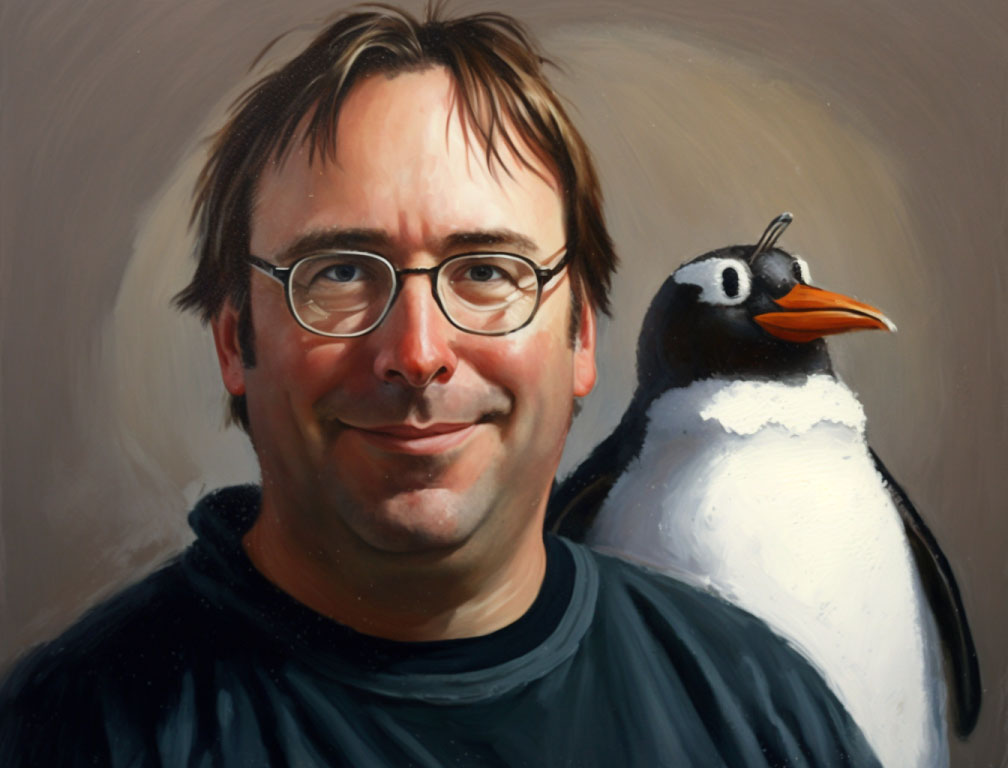
\includegraphics[width=0.4\textwidth]{./image/arithmetic/linux-torvalds-penguin-painting.jpg}
    \caption{Contoh Citra}
\end{figure}

Misalnya, dalam kasus menggunakan bahasa pemrograman Rust, kita dapat memanfaatkan library image untuk menerapkan operasi ini. Dalam contoh yang diberikan, terdapat sebuah citra yang akan dikalikan dengan sebuah maska 3x3 yang memiliki nilai-nilai identik, yaitu matriks yang berisi semua nilai 1. Proses ini dilakukan dengan iterasi melalui setiap piksel dalam citra, di mana nilai piksel tersebut akan dikalikan dengan nilai yang sesuai dalam maska, dan kemudian diambil rata-ratanya. Hasil akhirnya adalah citra baru yang mencerminkan efek visual yang lebih halus, menghasilkan kesan pengaburan atau \textit{blurring} yang dapat memberikan dimensi tambahan pada citra tersebut.

\begin{lstlisting}
use image::{open, GenericImageView, RgbaImage, Pixel};

fn main() {
    let penguin = open("linux-torvalds-penguin-painting.jpg").unwrap();
    let mask = [[1,1,1], [1,1,1], [1,1,1]];

    let (width, height) = penguin.dimensions();
    let mut result = RgbaImage::new(width, height);

    for x in 1..width-1 {
        for y in 1..height-1 {
            let mut r: i32 = 0;
            let mut g: i32 = 0;
            let mut b: i32 = 0;
            let mut a: i32 = 0;
            for i in 0usize..3 {
                for j in 0usize..3 {
                    let pixel = penguin.get_pixel(x+(i as u32)-1,
                                                    y+(j as u32)-1);
                    let channels = pixel.channels();
                    r = r.saturating_add((channels[0] * mask[i][j]).into());
                    g = g.saturating_add((channels[1] * mask[i][j]).into());
                    b = b.saturating_add((channels[2] * mask[i][j]).into());
                    a = a.saturating_add((channels[3] * mask[i][j]).into());
                }
            }
            result.put_pixel(x,
                                y,
                                image::Rgba(
                                    [(r/9).try_into().unwrap(),
                                        (g/9).try_into().unwrap(),
                                        (b/9).try_into().unwrap(),
                                        (a/9).try_into().unwrap()]));        }
    }

    result.save("result-multiplication.jpg").unwrap();
}
\end{lstlisting}


\begin{figure}[H]
    \centering
    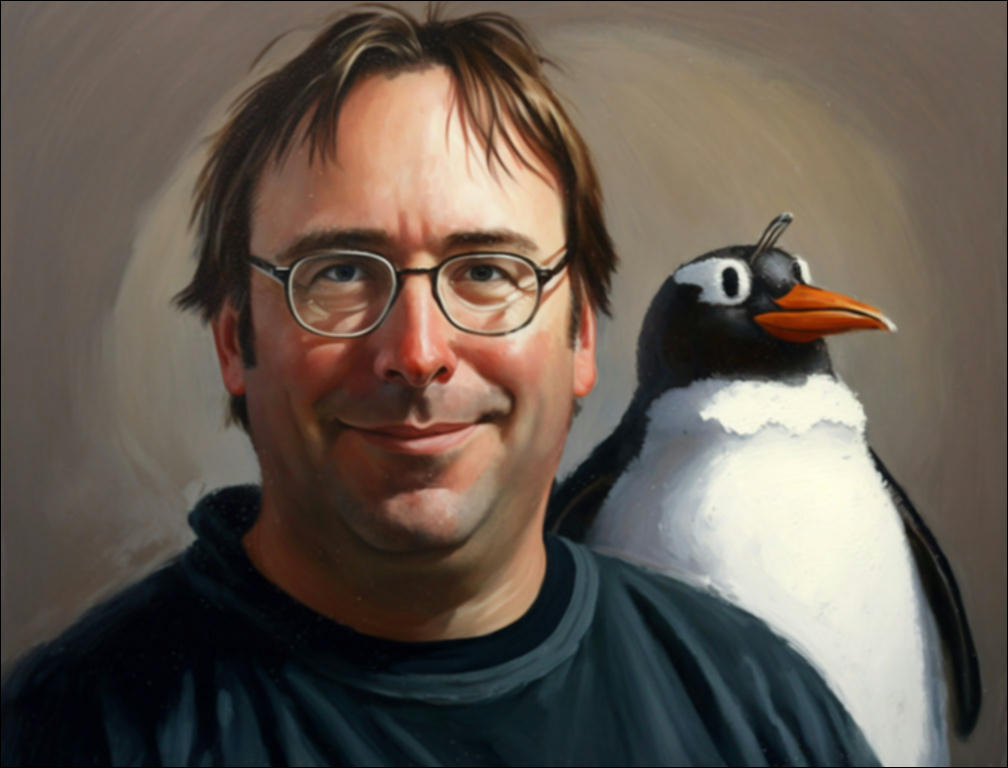
\includegraphics[width=0.4\textwidth]{./image/arithmetic/result-multiplication.jpg}
    \caption{Hasil Perkalian Citra}
\end{figure}
...

\subsection{Penjumlahan atau Pengurangan citra dengan nilai skalar}

Operasi penjumlahan atau pengurangan citra dengan nilai skalar memungkinkan kita untuk mengubah kontras dan kecerahan citra dengan cara yang fleksibel. Ini adalah teknik yang berguna dalam pengolahan gambar untuk menghasilkan efek visual yang diinginkan atau untuk meningkatkan kejelasan gambar. Saat menggunakan teknik ini, kita secara efektif menyesuaikan intensitas warna setiap piksel dalam citra dengan menambahkan atau mengurangkan nilai konstan. Dalam proses ini, setiap piksel diubah secara seragam, yang berarti perubahan kontras atau kecerahan diterapkan secara merata di seluruh citra.

\subsubsection{Contoh}
Misalnya, kita memiliki citra berikut:
\begin{figure}[H]
    \centering
    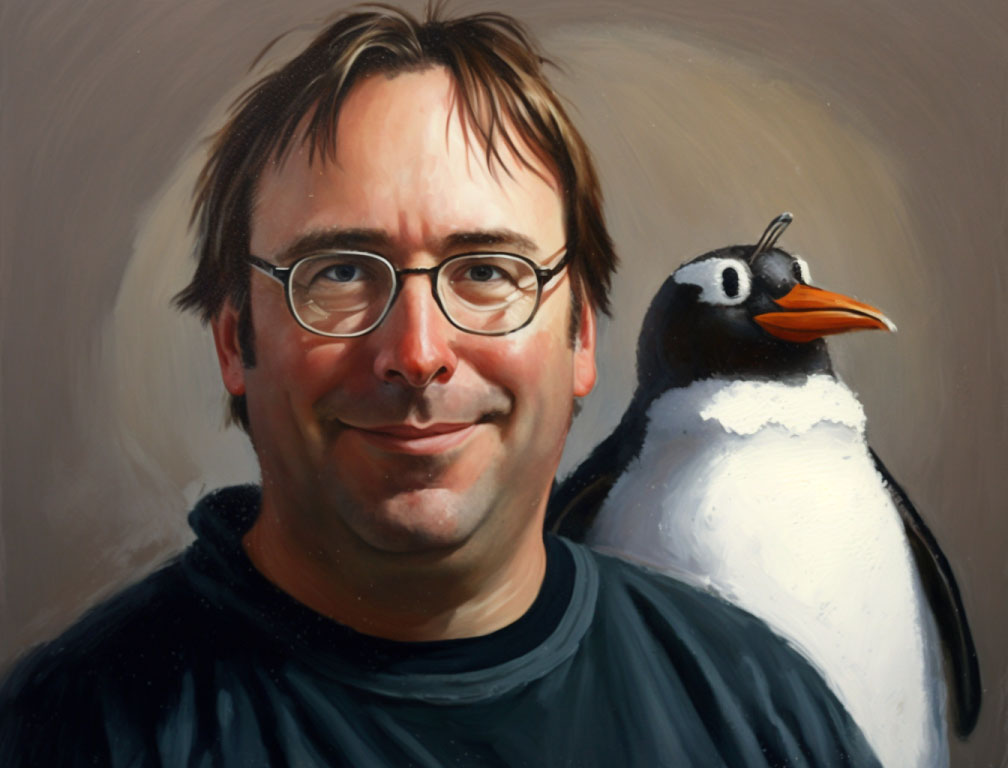
\includegraphics[width=0.4\textwidth]{./image/arithmetic/linux-torvalds-penguin-painting.jpg}
    \caption{Contoh Citra}
\end{figure}

\begin{lstlisting}
use image::{open, GenericImageView, RgbaImage, Pixel};

fn main() {
    let penguin = open("linux-torvalds-penguin-painting.jpg").unwrap();
    let scalar = 50;

    let (width, height) = penguin.dimensions();
    let mut result = RgbaImage::new(width, height);

    for x in 0..width {
        for y in 0..height {
            let pixel = penguin.get_pixel(x, y);
            let channels = pixel.channels();
            let r = (channels[0] as i32 + scalar).max(0).min(255) as u8;
            let g = (channels[1] as i32 + scalar).max(0).min(255) as u8;
            let b = (channels[2] as i32 + scalar).max(0).min(255) as u8;
            let a = channels[3];
            result.put_pixel(x, y, image::Rgba([r, g, b, a]));
        }
    }

    result.save("result-addition-scalar.jpg").unwrap();
}
\end{lstlisting}

Sebagai contoh, dalam kode Rust yang diberikan, kita memperoleh citra yang lebih terang dengan menambahkan nilai konstan ke setiap komponen warna (merah, hijau, dan biru) dari setiap piksel. Kemudian, untuk memastikan bahwa nilai-nilai yang dihasilkan tetap dalam rentang yang valid untuk nilai piksel (0 hingga 255), kita membatasi nilai-nilai tersebut. Hasilnya adalah gambar yang secara visual lebih cerah daripada citra aslinya, memberikan kesan yang lebih hidup dan menarik.

\begin{figure}[H]
    \centering
    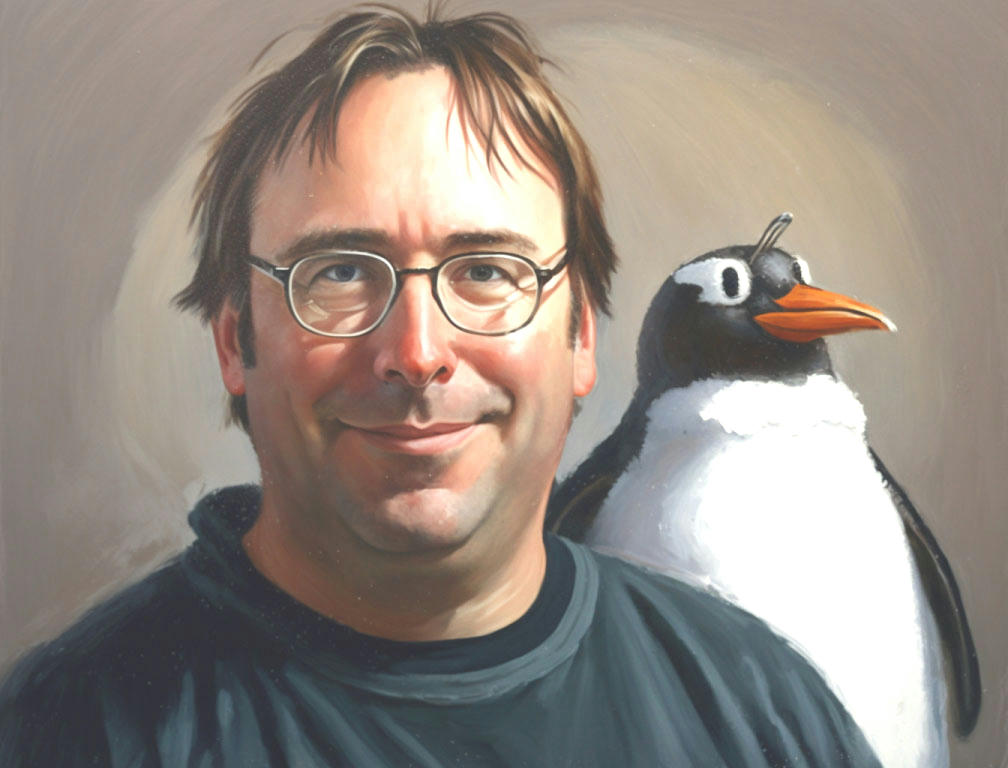
\includegraphics[width=0.4\textwidth]{./image/arithmetic/result-addition-scalar.jpg}
    \caption{Hasil Penjumlahan Citra dengan Nilai Skalar}
\end{figure}

Melalui pendekatan ini, kita memiliki kontrol yang lebih besar atas penyesuaian kontras dan kecerahan citra, memungkinkan kita untuk mencapai hasil yang diinginkan dengan mudah. Dalam praktiknya, teknik ini digunakan secara luas dalam berbagai aplikasi pengolahan gambar, mulai dari perbaikan gambar hingga pengolahan medis dan pengenalan pola. Dengan menggabungkan kreativitas dengan pemrograman, kita dapat menciptakan efek visual yang menarik dan memenuhi kebutuhan spesifik dari setiap proyek pengolahan gambar.

\subsection{Perkalian atau Pembagian citra dengan nilai skalar}
Perkalian atau pembagian citra dengan nilai skalar adalah teknik yang memungkinkan kita untuk secara efektif mengatur kontras dan kecerahan sebuah citra, serta menyesuaikan nilai piksel sesuai kebutuhan kita. Dalam dunia pemrosesan citra, kemampuan untuk mengontrol kontras dan kecerahan sangat penting untuk mencapai hasil akhir yang diinginkan. Bayangkan ini seperti mengedit foto di mana kita dapat meningkatkan atau mengurangi kecerahan untuk membuat gambar lebih menarik atau sesuai dengan tujuan yang diinginkan.

\subsubsection{Contoh}
Misalnya, kita memiliki citra berikut:

\begin{figure}[H]
    \centering
    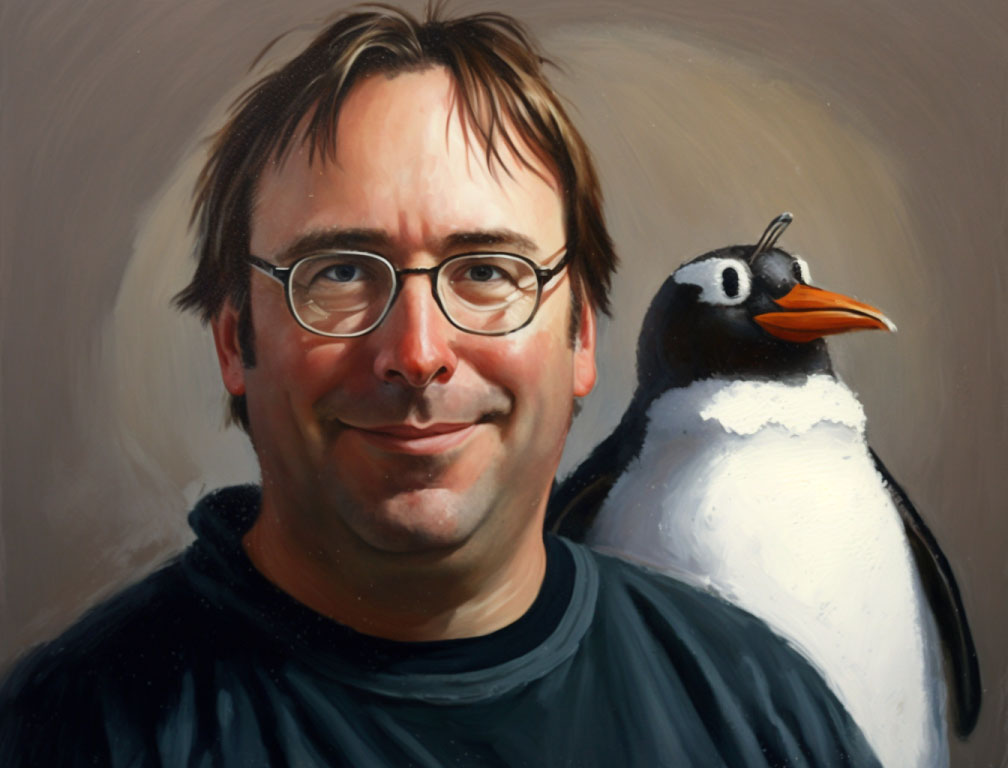
\includegraphics[width=0.4\textwidth]{./image/arithmetic/linux-torvalds-penguin-painting.jpg}
    \caption{Contoh Citra}
\end{figure}

Misalnya, ketika kita menggunakan teknik ini pada sebuah citra, kita mengalikan atau membagi nilai setiap piksel dalam citra dengan suatu konstanta. Ini berarti setiap titik dalam citra dipengaruhi secara seragam oleh operasi matematis yang sama. Dalam implementasi menggunakan Rust, kita menggunakan alat yang disebut \textit{Image Library} untuk memanipulasi citra secara programatik. Dengan kode yang sesuai, kita dapat melakukan operasi ini dengan mudah, memberikan kita kontrol penuh atas bagaimana citra kita akan diubah.

\begin{lstlisting}
use image::{open, GenericImageView, RgbaImage, Pixel};

fn main() {
    let penguin = open("linux-torvalds-penguin-painting.jpg").unwrap();
    let scalar = 0.5;

    let (width, height) = penguin.dimensions();
    let mut result = RgbaImage::new(width, height);

    for x in 0..width {
        for y in 0..height {
            let pixel = penguin.get_pixel(x, y);
            let channels = pixel.channels();
            let r = (channels[0] as f32 * scalar).max(0.0).min(255.0) as u8;
            let g = (channels[1] as f32 * scalar).max(0.0).min(255.0) as u8;
            let b = (channels[2] as f32 * scalar).max(0.0).min(255.0) as u8;
            let a = channels[3];
            result.put_pixel(x, y, image::Rgba([r, g, b, a]));
        }
    }

    result.save("result-multiplication-scalar.jpg").unwrap();
}
\end{lstlisting}

Kode di atas menggambarkan bagaimana kita dapat mengalikan atau membagi setiap piksel dalam citra dengan nilai konstan untuk mengatur kontras atau kecerahan citra. Dalam contoh ini, kita mengalikan setiap piksel dalam citra asli dengan nilai 0.5 untuk mengurangi kecerahan citra.

\begin{figure}[H]
    \centering
    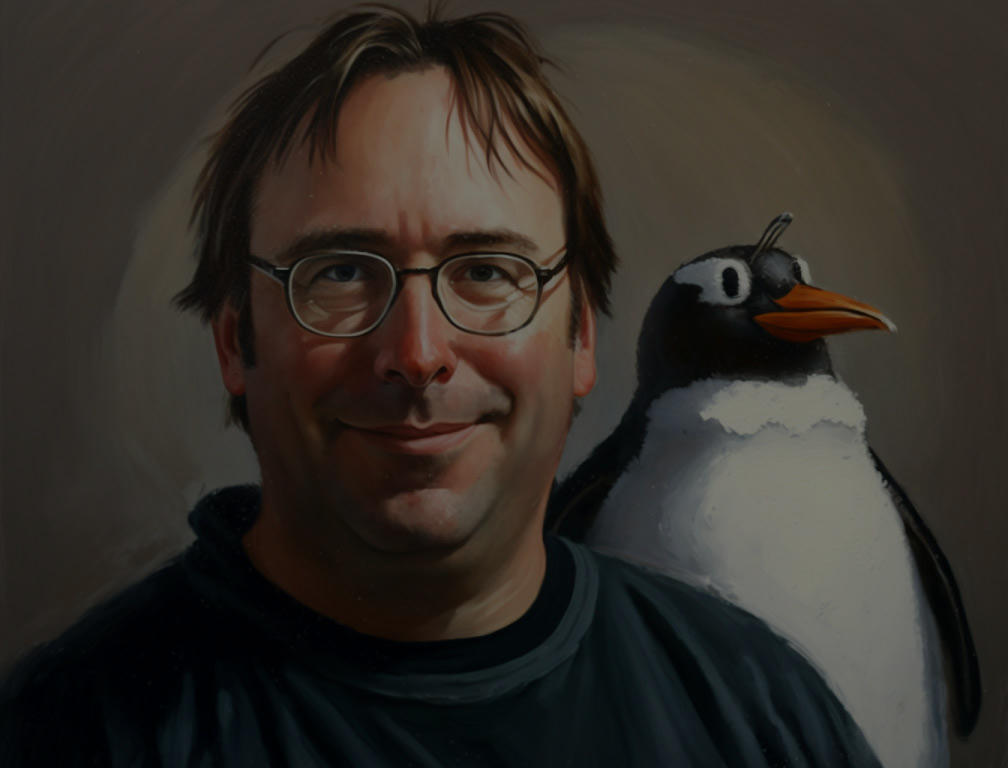
\includegraphics[width=0.4\textwidth]{./image/arithmetic/result-multiplication-scalar.jpg}
    \caption{Hasil Perkalian Citra dengan Nilai Skalar}
\end{figure}

\section{Penggunaan Operasi Logika (\textit{Bitwise})}
\subsection{Operasi AND}

Operasi AND merupakan salah satu alat dasar dalam pengolahan citra, terutama untuk membedakan kemiripan antara citra. Konsepnya terletak pada pemeriksaan piksel-piksel yang sesuai dari dua citra dan menghasilkan citra baru yang mencakup fitur-fitur yang mereka bagikan. Pada dasarnya, ini mirip dengan menimpa dua citra dan hanya menyimpan bagian yang tumpang tindih. Operasi ini banyak digunakan dalam tugas-tugas seperti segmentasi citra, di mana memisahkan elemen-elemen umum penting untuk analisis dan manipulasi.

Dalam implementasi praktisnya, menggunakan bahasa seperti Rust bersama dengan pustaka seperti image mempermudah proses tersebut secara signifikan. Dengan melakukan iterasi melalui setiap piksel dari citra masukan, operasi AND diterapkan pada saluran warna mereka, menghasilkan citra baru yang menyoroti karakteristik bersama mereka. Pendekatan ini memungkinkan pembuatan citra gabungan yang menyoroti area-area di mana kedua bentuk saling tumpang tindih. Sebagai contoh, menggabungkan citra berbentuk bintang dengan citra berbentuk lingkaran menggunakan operasi AND mengungkapkan daerah-daerah di mana kedua bentuk tersebut saling bertumpukan, memberikan wawasan tentang keberadaan spasial bersama mereka.

\subsubsection{Contoh}
Misalnya, kita memiliki dua citra berikut:
\begin{figure}[H]
    \centering
    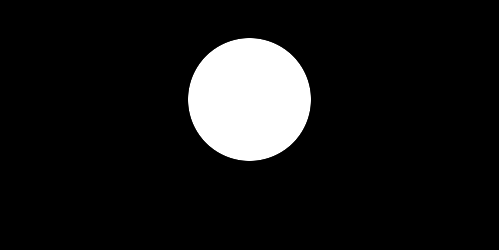
\includegraphics[width=0.4\textwidth]{./image/boolean/circle.png}
    
\includegraphics[width=0.4\textwidth]{./image/boolean/star-1.jpg}
    \caption{Contoh Citra}
\end{figure}

\begin{lstlisting}
fn and_operation(img_1: RgbaImage, img_2: RgbaImage) -> RgbaImage {
    let (width, height) = img_1.dimensions();

    let mut img = RgbaImage::new(width, height);

    for y in 0..height {
        for x in 0..width {
            let pixel_1 = img_1.get_pixel(x, y);
            let pixel_2 = img_2.get_pixel(x, y);

            let new_pixel = image::Rgba([
                pixel_1[0] & pixel_2[0],
                pixel_1[1] & pixel_2[1],
                pixel_1[2] & pixel_2[2],
                pixel_1[3] & pixel_2[3],
            ]);

            img.put_pixel(x, y, new_pixel);
        }
    }
    img
}
\end{lstlisting}

Menggunakan fungsi di atas, kita dapat melakukan operasi AND pada dua citra untuk menciptakan citra baru yang mewakili kesamaan antara keduanya. Dalam contoh ini, kita menggunakan citra bintang sebagai citra pertama dan citra lingkaran sebagai citra kedua. Hasilnya adalah citra baru yang mewakili kesamaan antara kedua citra tersebut.

\begin{figure}[H]
    \centering
    
\includegraphics[width=0.4\textwidth]{./image/boolean/output-and-operation.png}
    \caption{Hasil Operasi AND}
\end{figure}

\subsection{Operasi OR}


Operasi OR adalah prinsip sederhana dalam pengolahan citra yang memungkinkan kita untuk menggabungkan dua citra dengan cara yang menarik. Ketika kita berbicara tentang citra, kita melihatnya sebagai kumpulan piksel, dan operasi OR memungkinkan kita untuk menyatukan piksel-piksel dari dua citra untuk menciptakan citra baru yang mencerminkan kesamaan di antara keduanya. Ini seperti menyatukan dua dunia yang berbeda menjadi satu, di mana keberadaan suatu piksel dalam citra hasil adalah hasil dari ada atau tidak adanya piksel yang sesuai dalam kedua citra sumber.

Misalnya, bayangkan kita memiliki dua citra: satu berisi gambar bintang dan yang lainnya berisi gambar lingkaran. Melalui operasi OR, kita bisa menggabungkan keduanya sehingga citra hasilnya mencerminkan area yang ditutupi oleh baik bintang maupun lingkaran. Implementasi algoritma ini dengan bahasa pemrograman Rust menggunakan library image membuatnya menjadi tugas yang cukup sederhana. Namun, keajaiban sebenarnya terjadi ketika kita melihat citra baru yang dihasilkan. Itu adalah potongan baru dari dunia visual yang diciptakan melalui keseimbangan unik antara kedua citra sumber. Hasilnya adalah karya visual yang mengandung keunikan dan pesona dari gabungan elemen-elemen yang mungkin tidak akan kita temukan dalam satu citra tunggal.

\subsubsection{Contoh}
Misalnya, kita memiliki dua citra berikut:
\begin{figure}[H]
    \centering
    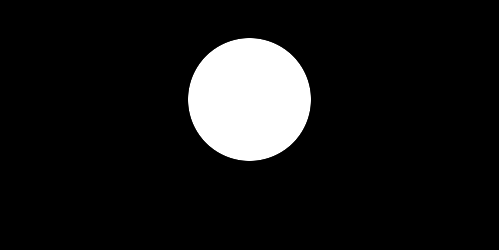
\includegraphics[width=0.4\textwidth]{./image/boolean/circle.png}
    
\includegraphics[width=0.4\textwidth]{./image/boolean/star-1.jpg}
    \caption{Contoh Citra}
\end{figure}

\begin{lstlisting}
fn or_operation(img_1: RgbaImage, img_2: RgbaImage) -> RgbaImage {
    let (width, height) = img_1.dimensions();

    let mut img = RgbaImage::new(width, height);

    for y in 0..height {
        for x in 0..width {
            let pixel_1 = img_1.get_pixel(x, y);
            let pixel_2 = img_2.get_pixel(x, y);

            let new_pixel = image::Rgba([
                pixel_1[0] | pixel_2[0],
                pixel_1[1] | pixel_2[1],
                pixel_1[2] | pixel_2[2],
                pixel_1[3] | pixel_2[3],
            ]);

            img.put_pixel(x, y, new_pixel);
        }
    }
    img
}
\end{lstlisting}


Dengan menggunakan fungsi yang telah diberikan, kita dapat dengan mudah melakukan operasi OR pada dua citra untuk menciptakan citra baru yang menampilkan kesamaan antara keduanya. Dalam contoh ini, kita menggunakan citra bintang sebagai citra pertama dan citra lingkaran sebagai citra kedua. Proses tersebut dilakukan dengan mengambil setiap piksel dari kedua citra, dan kemudian menerapkan operasi OR pada nilai piksel yang sesuai. Hasilnya adalah citra baru yang mencerminkan area yang tercakup oleh baik citra bintang maupun citra lingkaran. Dengan demikian, kita dapat melihat bagaimana kedua elemen visual tersebut bergabung menjadi satu dalam citra hasil, menciptakan representasi unik dari keduanya.

\begin{figure}[H]
    \centering
    
\includegraphics[width=0.4\textwidth]{./image/boolean/output-or-operation.png}
    \caption{Hasil Operasi OR}
\end{figure}

\subsection{Operasi NOT}

Operasi NOT, meskipun terlihat sederhana, memiliki signifikansi besar dalam pengolahan citra, terutama dalam menciptakan efek visual. Operasi ini menjadi elemen dasar dalam menciptakan negatif citra, di mana warna-warna dibalik untuk menghasilkan representasi yang kontras dari citra asli. Bayangkan sebuah kanvas digital di mana nilai setiap piksel mewakili sebuah warna atau bayangan. Dengan menerapkan operasi NOT pada nilai-nilai piksel ini, kita membaliknya, secara efektif mengubah hitam menjadi putih dan sebaliknya, serta mengubah seluruh spektrum warna sesuai. Dalam Rust, memanfaatkan pustaka seperti image mempermudah implementasi operasi ini, sehingga mudah bagi pengembang untuk memanipulasi citra dengan mudah.

\subsubsection{Contoh}
Misalnya, kita memiliki citra berikut:
\begin{figure}[H]
    \centering
    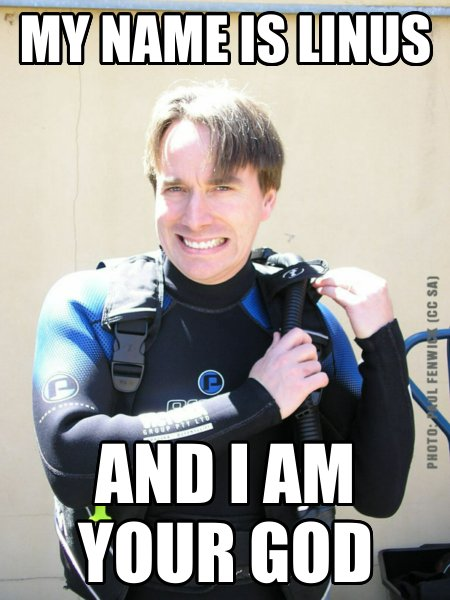
\includegraphics[width=0.4\textwidth]{./image/boolean/linus-meme.jpg}
    \caption{Contoh Citra}
\end{figure}

\begin{lstlisting}
fn not_operation(img: RgbaImage) -> RgbaImage {
    let (width, height) = img.dimensions();

    let mut new_img = RgbaImage::new(width, height);

    for y in 0..height {
        for x in 0..width {
            let pixel = img.get_pixel(x, y);

            let new_pixel = image::Rgba([
                !pixel[0],
                !pixel[1],
                !pixel[2],
                pixel[3],
            ]);

            new_img.put_pixel(x, y, new_pixel);
        }
    }
    new_img
}
\end{lstlisting}

Untuk memahami lebih dalam fungsinya, mari kita pertimbangkan contoh menggunakan implementasi Rust. Dalam potongan kode ini, setiap piksel dari sebuah citra mengalami transformasi, di mana saluran warnanya dibalik untuk menghasilkan efek negatif. Dengan menelusuri dimensi citra, piksel demi piksel, operasi NOT diterapkan, menghasilkan citra baru yang mencerminkan nada yang berlawanan dengan aslinya. Kemampuan ini membuka peluang untuk ekspresi kreatif, memungkinkan seniman dan pengembang untuk bereksperimen dengan kontras visual dan meningkatkan daya tarik estetika dari citra.

Diilustrasikan dengan meme Linus yang populer, citra hasilnya memperlihatkan kekuatan operasi NOT dalam mengubah representasi visual. Melalui proses ini, apa yang tadinya familiar berubah menjadi perspektif yang segar, menunjukkan potensi transformatif yang terkandung dalam operasi logika sederhana namun dalam, seperti NOT. Oleh karena itu, penerapan operasi semacam ini tidak hanya sekedar manipulasi; ia berfungsi sebagai katalisator untuk eksplorasi dan ekspresi artistik dalam ranah citra digital.


\begin{figure}[H]
    \centering
    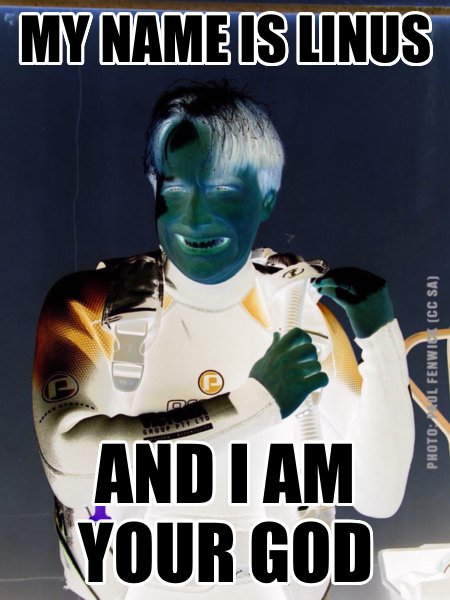
\includegraphics[width=0.4\textwidth]{./image/boolean/output-not-operation.png}
    \caption{Hasil Operasi NOT}
\end{figure}

\subsection{Operasi XOR}

Operasi XOR, yang merupakan singkatan dari exclusive OR, merupakan salah satu operasi logika yang paling dasar namun sangat penting dalam pengolahan citra. Keanggunannya terletak pada kesederhanaannya yang mengesampingkan pentingnya, karena operasi ini menjadi alat yang sangat kuat dalam menemukan kesamaan antara dua citra. Pada dasarnya, XOR bekerja dengan membandingkan nilai piksel dari dua citra, menghasilkan citra baru yang mencerminkan kesamaan di antara keduanya. Operasi ini memiliki berbagai aplikasi, mulai dari manipulasi citra hingga protokol kriptografi. Di dalam Rust, menggunakan pustaka Image untuk mempermudah proses implementasi, memfasilitasi eksekusi operasi XOR tanpa hambatan.

Contohnya, ada dua gambar yang berbeda: salah satunya menggambarkan sebuah lingkaran dan yang lainnya sebuah bintang. Dengan menerapkan operasi XOR menggunakan fungsi Rust yang disediakan, gambar baru muncul, secara visual menggambarkan unsur-unsur yang sama antara kedua gambar asli tersebut. Gambar hasilnya menampilkan gabungan fitur dari kedua gambar, mengungkapkan area di mana nilai pikselnya berbeda dan serupa. Melalui proses ini, pola-pola rumit dan detail dalam gambar ditekankan, menawarkan wawasan tentang komposisi dan perbedaan bersama mereka. Kemampuan seperti ini menegaskan peran operasi XOR dalam analisis dan sintesis gambar, melampaui kesederhanaannya untuk membuka pemahaman yang lebih dalam dalam data visual.

\subsubsection{Contoh}
Misalnya, kita memiliki dua citra berikut:
\begin{figure}[H]
    \centering
    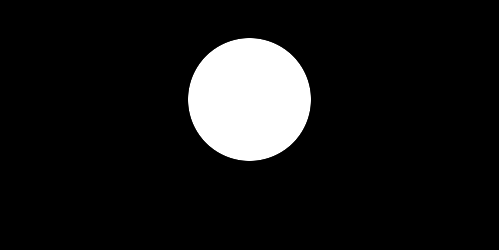
\includegraphics[width=0.4\textwidth]{./image/boolean/circle.png}
    
\includegraphics[width=0.4\textwidth]{./image/boolean/star-1.jpg}
    \caption{Contoh Citra}
\end{figure}

\begin{lstlisting}
fn xor_operation(img_1: RgbaImage, img_2: RgbaImage) -> RgbaImage {
    let (width, height) = img_1.dimensions();

    let mut img = RgbaImage::new(width, height);

    for y in 0..height {
        for x in 0..width {
            let pixel_1 = img_1.get_pixel(x, y);
            let pixel_2 = img_2.get_pixel(x, y);

            let new_pixel = image::Rgba([
                pixel_1[0] ^ pixel_2[0],
                pixel_1[1] ^ pixel_2[1],
                pixel_1[2] ^ pixel_2[2],
                !pixel_1[3] ^ pixel_2[3],
            ]);

            img.put_pixel(x, y, new_pixel);
        }
    }
    img
}
\end{lstlisting}

Menggunakan fungsi di atas, kita dapat melakukan operasi XOR pada dua citra untuk menciptakan citra baru yang mewakili kesamaan antara keduanya. Dalam contoh ini, kita menggunakan citra bintang sebagai citra pertama dan citra lingkaran sebagai citra kedua. Hasilnya adalah citra baru yang mewakili kesamaan antara kedua citra tersebut.

\begin{figure}[H]
    \centering
    
\includegraphics[width=0.4\textwidth]{./image/boolean/output-xor-operation.png}
    \caption{Hasil Operasi XOR}
\end{figure}

\section{Penggunaan Operasi Geometri}
\subsection{Rotasi Citra}
Rotasi citra adalah teknik penting dalam pengolahan citra yang memungkinkan kita untuk memutar citra sekitar titik tertentu. Ini adalah alat yang sangat berguna dalam berbagai aplikasi, dari pengolahan gambar medis hingga analisis citra satelit. Dalam Rust, menggunakan pustaka image mempermudah proses implementasi, memungkinkan kita untuk dengan mudah memanipulasi citra sesuai kebutuhan.

\subsubsection{Contoh}
Misalnya, kita memiliki citra berikut:
\begin{figure}[H]
    \centering
    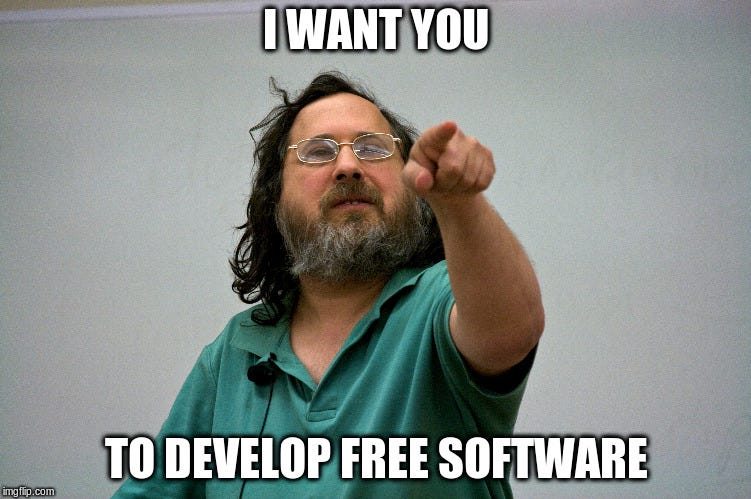
\includegraphics[width=0.4\textwidth]{./image/geometry/stallman-meme.jpg}
    \caption{Contoh Citra}
\end{figure}

\begin{lstlisting}
fn image_rotating(img: &RgbaImage, angle: f32) -> RgbaImage {
    let (width, height) = img.dimensions();
    let mut new_img = RgbaImage::new(width, height);
    let center_x = width as f32 / 2.0;
    let center_y = height as f32 / 2.0;
    for x in 0..width {
        for y in 0..height {
            let x_f32 = x as f32;
            let y_f32 = y as f32;
            let x_diff = x_f32 - center_x;
            let y_diff = y_f32 - center_y;
            let new_x = (x_diff * angle.cos() - y_diff * angle.sin() + center_x) as u32;
            let new_y = (x_diff * angle.sin() + y_diff * angle.cos() + center_y) as u32;
            if new_x < width && new_y < height {
                new_img.put_pixel(new_x, new_y, *img.get_pixel(x, y));
            }
        }
    }
    new_img
}
\end{lstlisting}

Dengan menggunakan fungsi di atas, kita dapat dengan mudah melakukan rotasi citra sesuai kebutuhan. Dalam contoh ini, kita menggunakan citra meme Stallman sebagai citra yang akan diputar. Hasilnya adalah citra baru yang mencerminkan rotasi citra asli sebesar sudut yang ditentukan.


\begin{figure}[H]
    \centering
    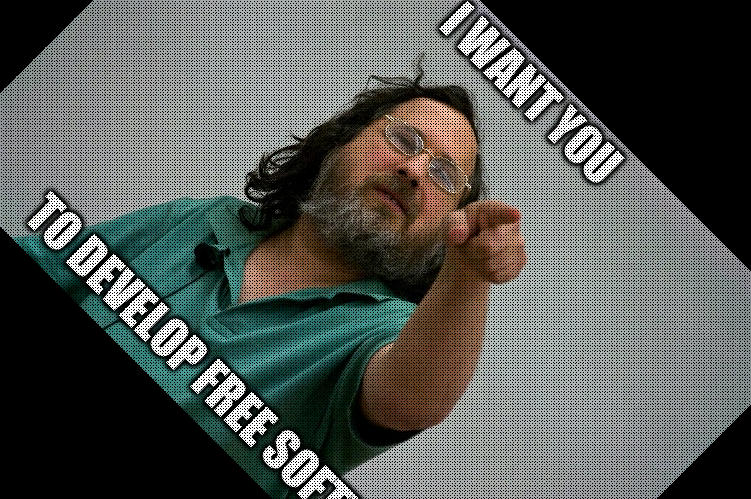
\includegraphics[width=0.4\textwidth]{./image/geometry/stallman-meme-rotated.jpg}
    \caption{Hasil Rotasi Citra}
\end{figure}


\subsection{Translasi Citra}
Translasi citra adalah salah satu teknik yang tak terpisahkan dalam dunia pengolahan citra, memungkinkan kita untuk memindahkan citra sepanjang sumbu x dan y. Teknik ini memiliki peran penting dalam berbagai aplikasi, mulai dari interpretasi gambar medis hingga analisis citra satelit yang kompleks. Dalam konteks pengembangan menggunakan bahasa pemrograman Rust, pustaka image menjadi sahabat yang handal untuk mempermudah implementasi, memungkinkan kita untuk dengan lancar memanipulasi citra sesuai kebutuhan.


\subsubsection{Contoh}
Misalnya, kita memiliki citra berikut:

\begin{figure}[H]
    \centering
    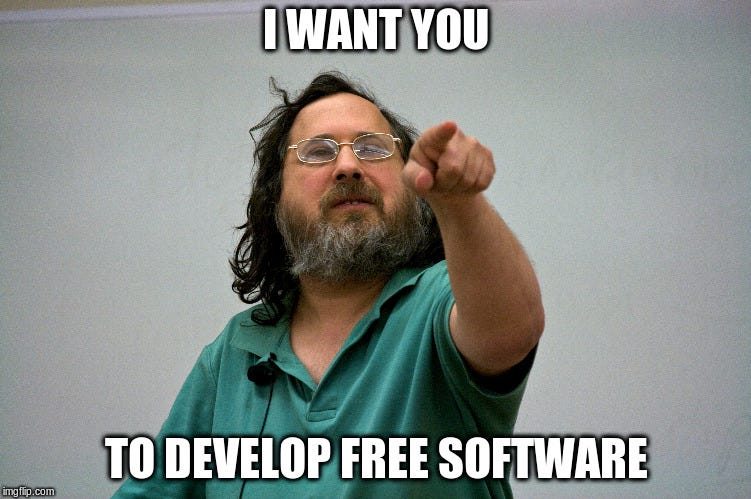
\includegraphics[width=0.4\textwidth]{./image/geometry/stallman-meme.jpg}
    \caption{Contoh Citra}
\end{figure}

\begin{lstlisting}
fn image_translating(img: &RgbaImage, x: i32, y: i32) -> RgbaImage {
    let (width, height) = img.dimensions();
    let mut new_img = RgbaImage::new(width, height);
    for i in 0..width {
        for j in 0..height {
            let new_x = i as i32 + x;
            let new_y = j as i32 + y;
            if new_x >= 0 && new_x < width as i32 && new_y >= 0 && new_y < height as i32 {
                new_img.put_pixel(new_x as u32, new_y as u32, *img.get_pixel(i, j));
            }
        }
    }
    new_img
}
\end{lstlisting}

Dengan menggunakan fungsi di atas, kita dapat dengan mudah melakukan translasi citra sesuai kebutuhan. Dalam contoh ini, kita menggunakan citra meme Stallman sebagai citra yang akan dipindahkan. Hasilnya adalah citra baru yang mencerminkan translasi citra asli sebesar nilai x dan y yang ditentukan.

\begin{figure}[H]
    \centering
    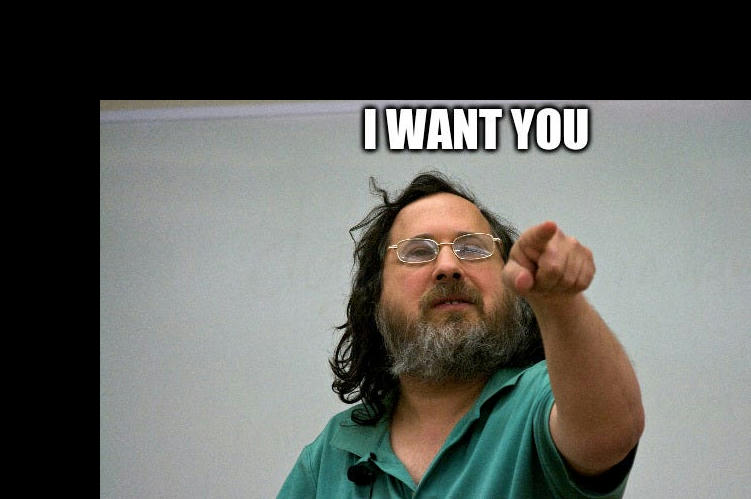
\includegraphics[width=0.4\textwidth]{./image/geometry/stallman-meme-translated.jpg}
    \caption{Hasil Translasi Citra}
\end{figure}

\subsection{Flip Citra}

Flip citra adalah salah satu teknik krusial dalam dunia pengolahan citra yang memungkinkan kita untuk membalik citra sepanjang sumbu x atau y. Teknik ini terbukti sangat berguna dalam berbagai aplikasi, mulai dari diagnosa medis hingga pemetaan citra satelit. Dalam lingkungan bahasa pemrograman Rust, penggunaan pustaka image menjadi landasan yang kokoh untuk melaksanakan proses ini dengan mudah, memberikan kemudahan dalam memanipulasi citra sesuai kebutuhan.


\subsubsection{Contoh}
Misalnya, kita memiliki citra berikut:

\begin{figure}[H]
    \centering
    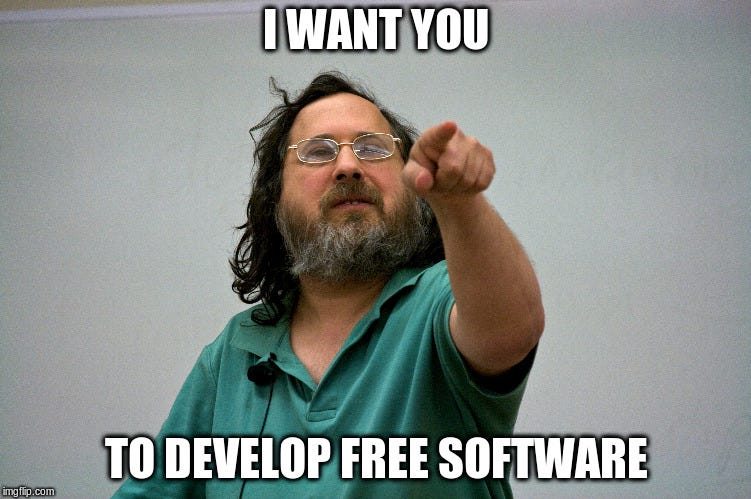
\includegraphics[width=0.4\textwidth]{./image/geometry/stallman-meme.jpg}
    \caption{Contoh Citra}
\end{figure}

\begin{lstlisting}
fn image_flip(img: &RgbaImage, horizontal: bool, vertical: bool)
-> RgbaImage {
    let mut new_img = img.clone();
    match (horizontal, vertical) {
        (true, false) => {
            for x in 0..img.width() {
                for y in 0..img.height() {
                    let pixel = img.get_pixel(x, y);
                    new_img.put_pixel(img.width() - x - 1, y, *pixel);
                }
            }
        }
        (false, true) => {
            for x in 0..img.width() {
                for y in 0..img.height() {
                    let pixel = img.get_pixel(x, y);
                    new_img.put_pixel(x, img.height() - y - 1, *pixel);
                }
            }
        }
        (true, true) => {
            for x in 0..img.width() {
                for y in 0..img.height() {
                    let pixel = img.get_pixel(x, y);
                    new_img.put_pixel(img.width() - x - 1, img.height() - y - 1, *pixel);
                }
            }
        }
        (false, false) => {
            return new_img;
        }
    }

    new_img
}
\end{lstlisting}

Dengan menggunakan fungsi di atas, kita dapat dengan mudah melakukan proses flip citra sesuai dengan parameter yang telah ditentukan. Dalam contoh ini, kita menggunakan citra meme Stallman sebagai objek flip. Hasilnya adalah citra baru yang mencerminkan flip citra aslinya, entah itu sepanjang sumbu x, sumbu y, atau keduanya, sesuai kebutuhan.

\begin{figure}[H]
    \centering
    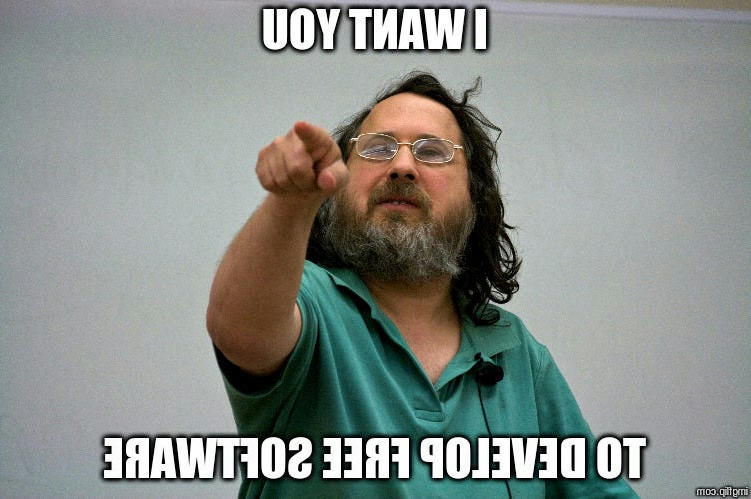
\includegraphics[width=0.4\textwidth]{./image/geometry/stallman-meme-flipped-x.jpg}
    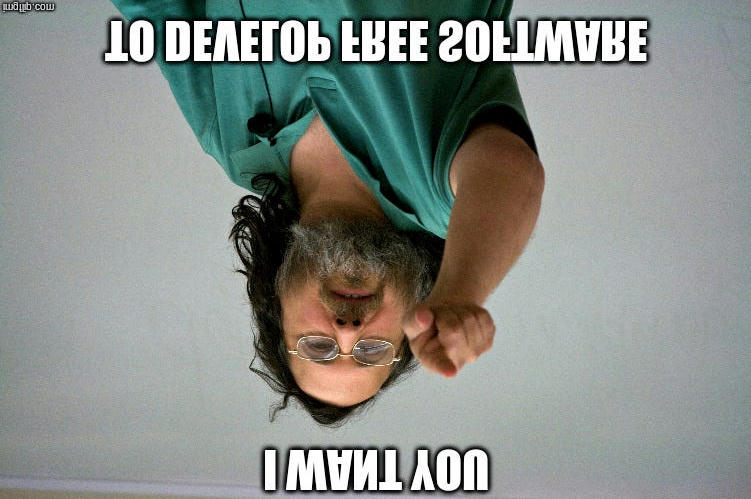
\includegraphics[width=0.4\textwidth]{./image/geometry/stallman-meme-flipped-y.jpg}
    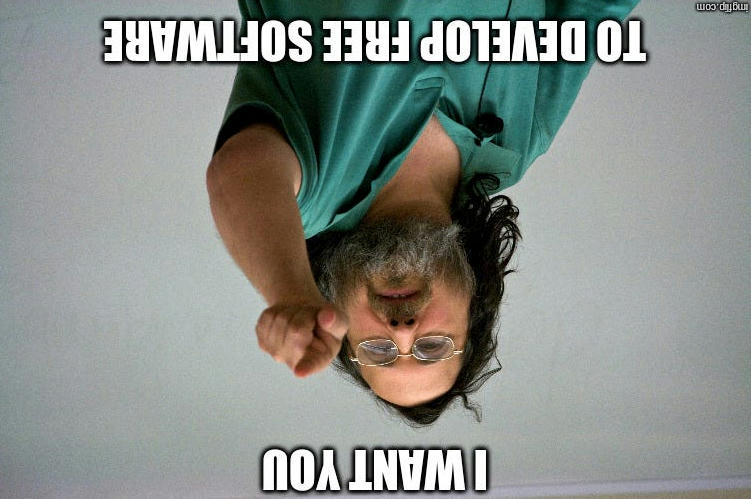
\includegraphics[width=0.4\textwidth]{./image/geometry/stallman-meme-flipped-xy.jpg}
    \caption{Hasil Flip Citra}
\end{figure}

\subsection{Skala Citra}

Skala citra adalah suatu teknik yang sangat vital dalam domain pengolahan citra, memungkinkan kita untuk memperbesar atau memperkecil citra dengan proporsi yang diinginkan. Keberadaannya meluas dalam beragam aplikasi, dari dunia medis dengan pengolahan gambar hingga analisis citra satelit yang kompleks. Dalam konteks bahasa pemrograman Rust, penggunaan pustaka image menjadi kunci dalam memudahkan implementasi teknik ini, memberikan akses yang lancar untuk memanipulasi citra sesuai dengan kebutuhan.

\subsubsection{Contoh}
Misalnya, kita memiliki citra berikut:

\begin{figure}[H]
    \centering
    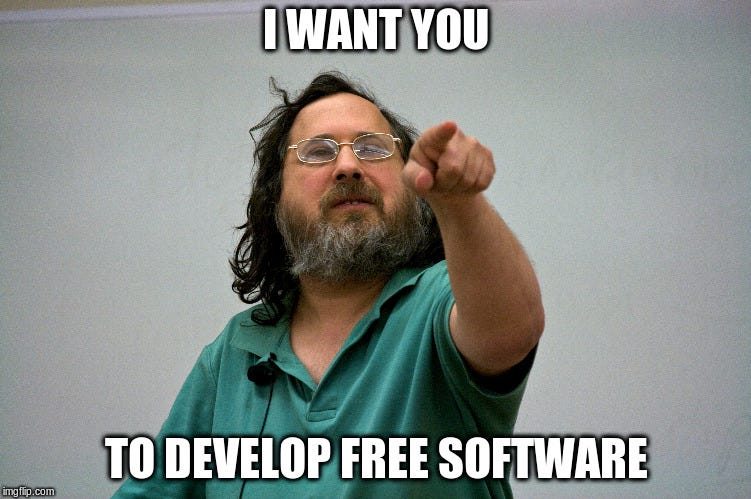
\includegraphics[width=0.4\textwidth]{./image/geometry/stallman-meme.jpg}
    \caption{Contoh Citra}
\end{figure}

\begin{lstlisting}
fn image_zooming(img: &RgbaImage, factor: f32) -> RgbaImage {
    let (width, height) = img.dimensions();
    let new_width = (width as f32 * factor) as u32;
    let new_height = (height as f32 * factor) as u32;
    let mut new_img = RgbaImage::new(new_width, new_height);
    for x in 0..new_width {
        for y in 0..new_height {
            let old_x = (x as f32 / factor) as u32;
            let old_y = (y as f32 / factor) as u32;
            if old_x < width && old_y < height {
                new_img.put_pixel(x, y, *img.get_pixel(old_x, old_y));
            }
        }
    }
    new_img
}
\end{lstlisting}


Dengan menggunakan fungsi di atas,  kita dapat dengan mudah melakukan proses skala citra sesuai dengan parameter faktor yang diinginkan. Melalui contoh ini, kita memperoleh citra baru yang mencerminkan skala citra aslinya, disesuaikan dengan faktor yang telah ditentukan.

\begin{figure}[H]
    \centering
    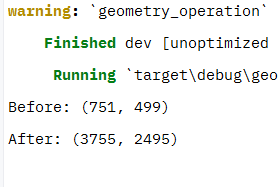
\includegraphics[width=0.4\textwidth]{./image/geometry/image_zoom_res.png}
    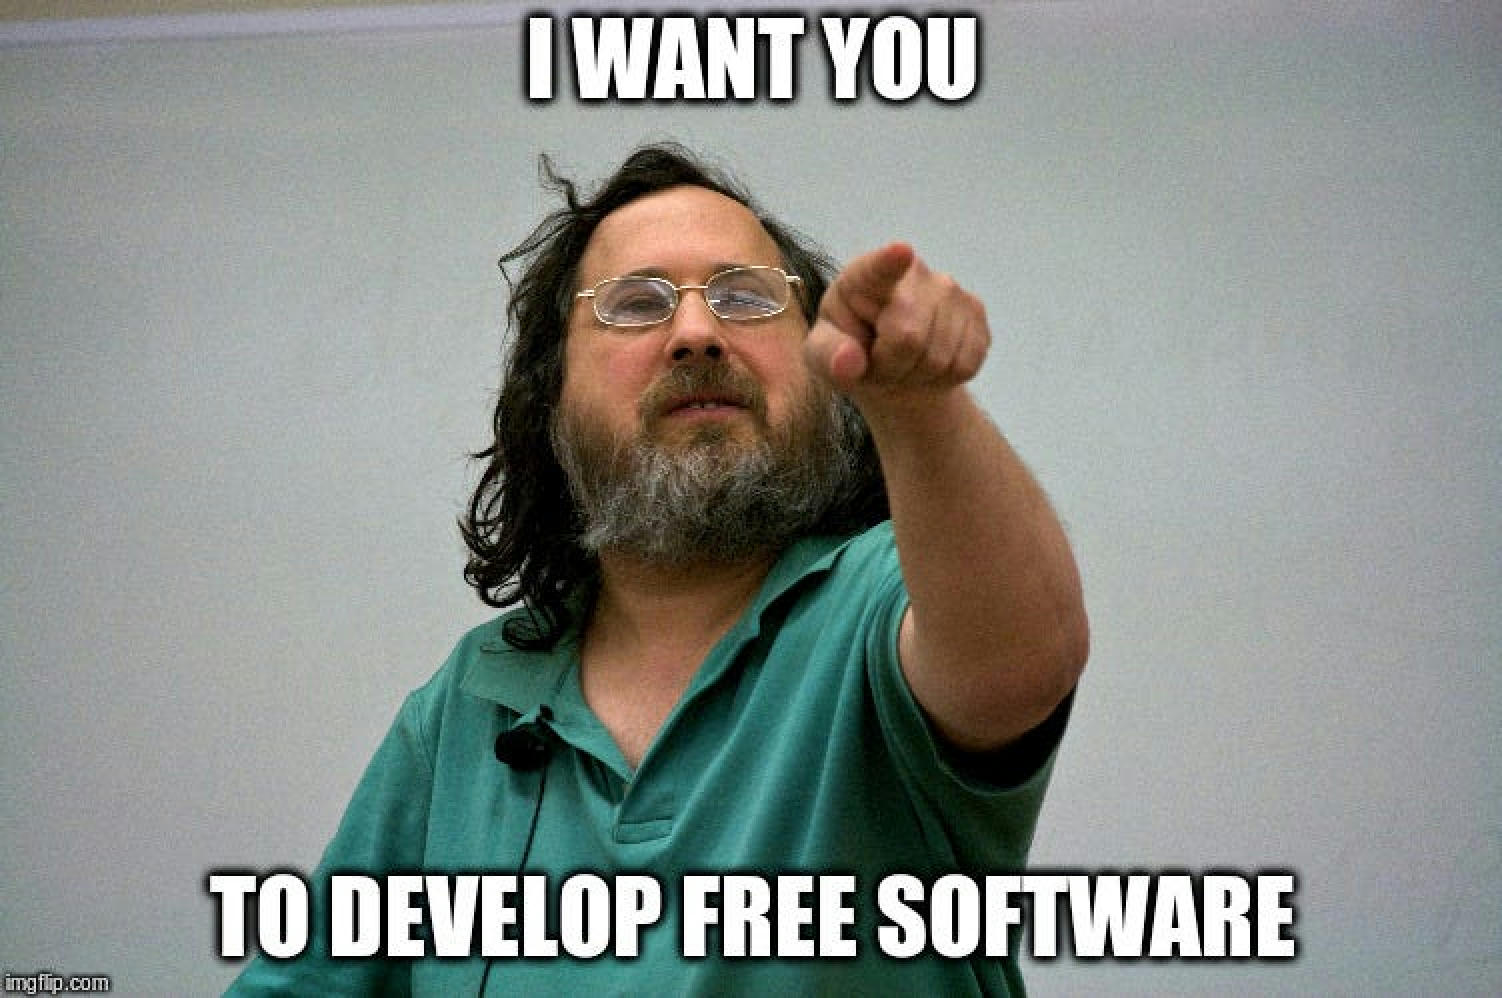
\includegraphics[width=0.4\textwidth]{./image/geometry/stallman-meme-zoomed.jpg}
    \caption{Hasil Skala Citra dan Detail Resolusi Hasil Skala}
\end{figure}

\chapter{Penutup}

Dengan demikian, kita telah menjelajahi berbagai teknik pengolahan citra yang dapat diimplementasikan menggunakan bahasa pemrograman Rust. Dari operasi aritmatika hingga operasi logika, dari operasi geometri hingga teknik lainnya, kita telah melihat bagaimana Rust dapat digunakan untuk memanipulasi citra dengan mudah dan efisien. Dengan pustaka seperti image, kita memiliki alat yang kuat untuk memanipulasi citra sesuai kebutuhan, membuka peluang untuk eksplorasi kreatif dan inovasi dalam pengolahan citra.

Pengetahuan yang diperoleh dari eksplorasi ini dapat diterapkan dalam berbagai aplikasi, mulai dari pengolahan gambar medis hingga analisis citra satelit. Dengan kreativitas dan pemrograman, kita dapat menciptakan efek visual yang menarik dan memenuhi kebutuhan spesifik dari setiap proyek pengolahan gambar. Dengan demikian, Rust menjadi alat yang kuat dalam pengolahan citra, membuka peluang untuk eksplorasi kreatif dan inovasi dalam pengolahan citra. Untuk repositori kode lengkap, silakan kunjungi \url{https://github.com/elskow/image-processing/tree/main/3-basic-operation-image}.

\renewcommand{\bibname}{Daftar Pustaka}
\begin{thebibliography}{9}
    \addcontentsline{toc}{chapter}{Daftar Pustaka}

    \bibitem{rust-lang}
    The Rust Programming Language. (n.d.). Retrieved from \url{https://www.rust-lang.org/}

    \bibitem{image-crate}
    Image. (n.d.). Retrieved from \url{https://crates.io/crates/image}

    \bibitem{burger-burge}
    Burger, W., Burge, M. J. (2009). Principles of Digital Image Processing: Core Algorithms (Undergraduate Topics in Computer Science) (2009th ed.). Springer.

    \bibitem{gonzalez-woods}
    Gonzalez, R. C., Woods, R. E. (2017). Digital Image Processing (4th ed.). Pearson.

\end{thebibliography}

\end{document}